\documentclass[Report.tex]{subfiles}
\externaldocument[I-]{chapter_1_introduction.tex}
\externaldocument[M-]{chapter_2_method.tex}
\externaldocument[D-]{chapter_3_discardMethod.tex}
\externaldocument[R-]{chapter_4_result.tex}
\externaldocument[C-]{chapter_5_conclusion.tex}

\begin{document}
\chapter{Recognition}
\label{chap:Recognition}
\section{Background Knowledges}
\subsection{CNN - Basics}
\label{Recognition:subsec:MLP}
\begin{flushleft}
  AS mention i section \ref{Method:Classification} CNN have a few component to tune. Here we list up them and discuss the different component of a CNN.

  \begin{itemize}
    \item{Convolutional layer}
    \begin{itemize}
      \item{This layer consists of several filters/kernels that are convolved over the image and based on how many filters one uses, the same amount of feature images are made. The purpose of the filters are to grasp some spatial characteristics of the image, and make it available for further processing.
      The filters here correspond to the weights in the MLP, these are first initialized at random (or with a smart initialization method), then these will be updated as the network is trained.
      First layer filters are able to spot simple geometry like straight or curved lines, but the deeper we dive into networks topology the more complex shapes the filters can recognize. It is not unusual that last layers on large networks can differentiate between faces, animals, objects.\par
      In a CNN we can have arbitrary many convolutional layer and arbitrary many filters at each layer. However just like a regular MLP, increasing the number of layers and or filters; can allow the network to fit the training data arbitrarily well, unfortunately at the cost of processing time, mostly during training, but also during prediction phase.}
    \end{itemize}
    \item{Pooling}
    \begin{itemize}
      \item{The pooling layer allows us to downsize the data. This makes it possible to start with images which are relatively big, and as it's data propagates through the network we downsize it. As for the convolution layer the pooling layer can be used arbitrarily many times in a network.
      Pooling makes our network rotation invariant to minor changes in angle, as outputs max/min value of a (pooling-size) block regardless of where in the block this value is.}
    \end{itemize}
    \item{Fully connected layers (FC)}
    \begin{itemize}
      \item{This layer works basically the same way as the hidden layers in an MLP.
      The output of last convolution layer is then flattened and send to N fully connected layers (also sometimes referenced as dense layer). At the last layer we have same number of outputs as we have classes, just like in regular MLP.}
    \end{itemize}
  \end{itemize}
\end{flushleft}


  \begin{flushleft}
    \subsection{Deep Neural Network}
    \label{Recognition:subsec:MLP}
    Multilayer perceptron neural networks are relatively straight
    forward to code, however the challenging part is to decide on good hyper-parameters and to not overfit our network. \par
    Research has shown that the choices of parameters can have huge effects on the error rate through empirical testing. As empirical testing has shown that some combinations of parameters are better than others, we will also use the same method to find decent values on several of the hyper-parameters. More on this bellow, where a short description of the hyper-parameters follow. \par
    One obvious disadvantage we might face by using MLP is that slight spatial change on where in the image the characters are located, might lead to characters classified differently. This is because there is no spatial connections on a MLP, or rather MLP can't connect same object on the image but slightly shifted to right/left as it appears like completely different objects due to the fact MLP is build up.
  \end{flushleft}

  \begin{figure}[H]
    \centering
    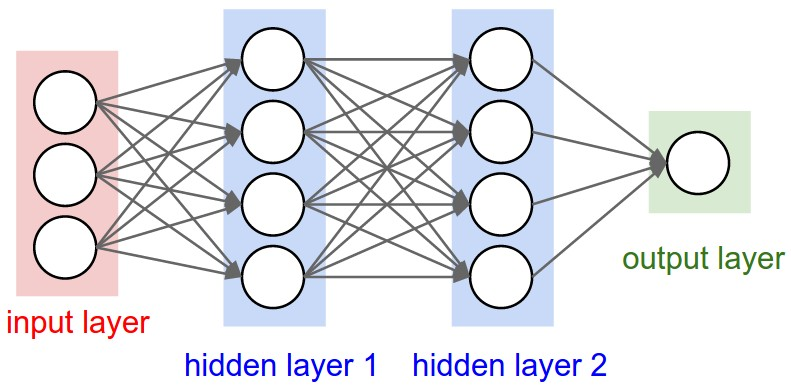
\includegraphics[height=4cm]{res/neural_net2.jpeg}
    \caption{MLP Neural network \href{http://cs231n.github.io/neural-networks-1/}{Source}}
    \label{fig:neural_net2}
  \end{figure}


  \begin{flushleft}
    \textbf{Hyper-parameters}
    \begin{itemize}
     \item{Number of hidden layers}
     \begin{itemize}
      \item{Layers decide how well the software can define the decision borders. Hence increase in layers can have a positive effect, there are also cons with the amount of layers. The more layers, the greater the computational power needed to train the system. We will be using the empirical method to decide how many layers we need}
     \end{itemize}
     \item{Number of nodes in each hidden layer}
     \begin{itemize}
      \item{Nodes in each hidden layer has the same effect as the number of hidden layers, hence the same applies for this hyper-parameter.}
     \end{itemize}
     \item{Activation functions}
     \begin{itemize}
      \item{The activation function decides which combination of nodes, with their signals, are allowed to propagate through the network. Here we will be using the \textit{rectified linear unit} (RELU) activation function. This is an activation function that allows propagation if the signal is positive, otherwise it will forward a zero. The reason for choosing this activation function is because this function handles the \textit{vanishing gradient problem} better than sigmoid and a tanh activation functions. More on vanishing gradient problem under ``optimization function''.}
     \end{itemize}
     \item{Loss function}
     \begin{itemize}
      \item{The loss function describes how far off the predicted class of the character is from the real class. In our case since we have multiple classes and we are going to use \textit{softmax regression} as the output layer, we also will be using the \textit{cross-entropy loss function}.}
     \end{itemize}
     \item{Optimization function}
     \begin{itemize}
      \item{The backpropagation will train the weights by Gradient Decent Optimization. However as training with several thousand examples, and then optimizing the weights and run the training process, is too costly resource wise, we will have to implement the \textit{mini-batch gradient decent optimization}. Same principle as gradient decent optimization, but this way we will find the gradient decent for each batch. As long as these batches are randomly chosen, and the sizes are large enough, (we will be using 100 as batch size), these will represent the entire dataset well enough.}
     \end{itemize}
     \item{Learning rate}
     \begin{itemize}
      \item{Learning rate is a scalar that decides how large the steps towards the gradient minimum will be, for the weights. Choosing too small of a learning-rate we might risk not reaching the bottom of the graph, we also might get stuck in a local minimum. Choosing too large of a learning rate we might risk never settle down on a minimum. \par
      For the learning rate we will be using the empirical method too.}
     \end{itemize}
     \item{Initialization of the weights and biases}
     \begin{itemize}
      \item{Initialization of the weights also seems to be of importance, researchers have found out. This is obvious, as for example setting all the weights to zero, would of course lead to a network with very few active nodes. \par
      We will be using the initialization of zeros for the biases, not any apparent reason. Based on our research, it seems people have gotten decent results when using this initialization. For the weights we will be using a Gaussian distribution, mean=0, standard deviation=1. Again this is also something that we have read should be a good initialization for the weights, no other reason.}
     \end{itemize}
     \item{Number of epochs}
     \begin{itemize}
      \item{Number of epochs are only relevant when we have a small number of dataset. When we have a small dataset we might want to run the software on the same dataset several times. This might result in overfitting the software to the dataset, therefore it is really important to be careful of the number of epochs, in cases with small datasets.}
     \end{itemize}
    \end{itemize}
  \end{flushleft}


\section{Datasets}
\section{Code used}
\section{articles}

%\begin{itemize}
% \item{}
%\end{itemize}

\end{document}
